\documentclass[11pt,a4paper]{letter}
\usepackage[top=0.50in, bottom=0.5in, left=1.1in, right=1.1in]{geometry}
\usepackage{graphicx}

%\signature{}

\usepackage{Sweave}
\begin{document}

\begin{letter}{}

\includegraphics[width=0.3\textwidth]{logo_uah.png}

\opening{Dear Dr. Armarego-Marriot:} % EMW14Oct  -- I think you can address to the editor you've been corresponding with (but not critical). %IMC15OCT done

\noindent Please consider our revised manuscript `Phylogenetic estimates of species-level phenology improve ecological forecasting' as an Article in \emph{Nature Climate Change}. This manuscript proposes a novel approach to incorporating phylogenetic relationships into models aimed at ecological forecasting. Results from our phenology-based case study demonstrate that this approach significantly enhances forecast accuracy.


\vspace{1.5ex}\\
\noindent We have edited our manuscript to acknowledge more clearly how our approach is preferable to others, emphasizing the benefits of fitting a Bayesian phylogenetic mixed model (PMM), as requested by reviewer \#3. In response to reviewer \#3, we have also incorporated RMSE as an additional metric for evaluating prediction accuracy in our cross-validation analysis, with results reinforcing our previously submitted conclusions. Finally, we have made minor corrections (e.g., legend of Fig. S9) and small edits to the text to meet NCC format standards. We believe these changes both strengthen the manuscript and address the reviewer's concerns. 


\vspace{1.5ex}\\
\noindent We detail our changes, point-by-point, in the following pages (note that reviewer comments are in \emph{italics}, while our responses are in regular text). The main text of our revised manuscript has 5,260 words including methods and legends, it has 54 references and contains 4 figures. This manuscript is not under consideration elsewhere.  We hope that you will find it suitable for publication in \emph{Nature Climate Change}, and look forward to hearing from you.
\vspace{2.5ex}\\



\vspace{1.5ex}\\
\noindent Sincerely,\\
\vspace{1.5ex}\\
 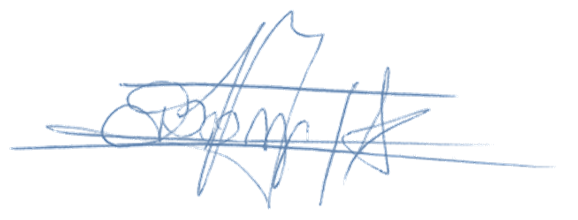
\includegraphics[width=0.2\textwidth]{Signature_IMC.png} \\
 \vspace{1.5ex}\\
\noindent Ignacio Morales-Castilla


\clearpage
\noindent Authors:\\
Ignacio Morales-Castilla,$^{1}$ T. J. Davies,$^{2,3}$ Geoffrey Legault,$^{3}$ D. M. Buonaiuto,$^{4,5,6}$ Catherine J. Chamberlain,$^{4,5,7}$ Ailene K. Ettinger,$^{5,8}$ Mira Garner,$^{3}$ Faith A. M. Jones,$^{3,10}$ Deirdre Loughnan,$^{3}$ William D. Pearse,$^{11}$ Darwin S. Sodhi$^{3}$ \& E. M. Wolkovich$^{3,4,5}$  \vspace{2ex}\\
\emph{Author affiliations:}\\
$^{1}$GloCEE - Global Change Ecology and Evolution Group, Department of Life Sciences, University of Alcal\'a, Alcal\'a de Henares, Spain\\ % (ORCID: 0000-0002-8570-9312)
 $^{2}$Botany, Faculty of Sciences, University of British Columbia, 2424 Main Mall, Vancouver, BC V6T 1Z4, Canada\\
$^{3}$Forest \& Conservation Sciences, Faculty of Forestry, University of British Columbia, 2424 Main Mall, Vancouver, BC V6T 1Z4, Canada\\
$^{4}$Organismic \& Evolutionary Biology, Harvard University, 26 Oxford Street, Cambridge, Massachusetts, USA\\
$^{5}$Arnold Arboretum of Harvard University, 1300 Centre Street, Boston, Massachusetts, USA\\
$^{6}$Department of Environmental Conservation, University of Massachusetts-Amherst, 160 Holdsworth Way, Amherst, MA, USA\\  % 01003
 $^{7}$The Nature Conservancy, 334 Blackwell St Ste 300, Durham, NC, USA \\ %27701
$^{8}$The Nature Conservancy of Washington, 74 Wall Street, Seattle, WA  USA \\ % 98121
$^{10}$Department of Wildlife, Fish and Environmental Studies, Swedish University of Agricultural Sciences, 901 83 Umea, Sweden\\ % Faith
$^{11}$Department of Life Sciences, Imperial College London, Silwood Park, Ascot, Berkshire, SL5 7PY, UK\\



\end{letter}
\end{document}
